\documentclass[a4paper]{article}

\usepackage[english]{babel}
\usepackage[utf8]{inputenc}
\usepackage{fullpage}
\usepackage{amsmath}
\usepackage{graphicx}
\usepackage[colorinlistoftodos]{todonotes}
\usepackage{hyperref}
\usepackage{amssymb}
\usepackage{outline} \usepackage{pmgraph} \usepackage[normalem]{ulem}
\usepackage{graphicx} \usepackage{verbatim}
% \usepackage{minted} % need `-shell-escape' argument for local compile

\title{
    \vspace*{1in}
    
\includegraphics[width=2.75in]{figures/UCAS-LOGO.png} \\
    \vspace*{1.2in}
    \textbf{\huge Weekly Work Report}
    \vspace{0.2in}
}

\author{Author Name \\
    \vspace*{0.5in} \\
    \textbf{LeiChao} \\
    \vspace*{1in}
}

\date{\textbf{2021-08-[02, 08]}}


\begin{document}

\maketitle
\setcounter{page}{0}
\thispagestyle{empty}
\newpage


\section{Gurobi Practise}

\subsection{Cash-Flow Matching Problem}
Cash-flow mastching is a investment strategy which could be wilded by investor to manage their future available cash-flow. In a other word, CASH-Flow Matching is a structure investment portfolio.

\subsection{Modeling Cash-Flow Problem}
Assuming A cooporation's cash flow requirement showed in \ref{fig:cash-flow-requirement}.

\begin{figure}[h]
    \centering
    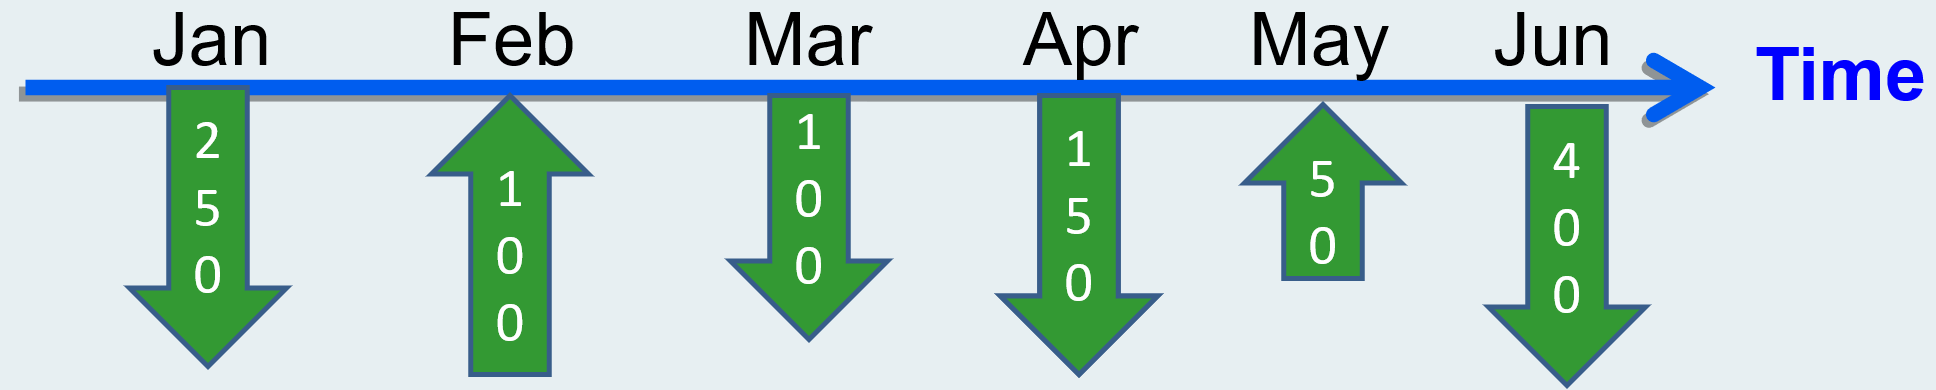
\includegraphics[width=0.75\textwidth]{figures/cash-flow-requirement.png}
    \caption{Cash-flow-requirement}
    \label{fig:cash-flow-requirement}
\end{figure}

A Corp has three kinds of invesment options.

\begin{description}
    \item[option 1] Get a loan up to 150w which need to pay 1.5\% per month interest from bank at the start of the month.
    \item[option 2] A corp could sell its 60-days commercial paper to the public, the total interest is 2\%.
    \item[option 3] A invest the rest of the money of last month in a stable 0.5\% interest per month.
\end{description}

\subsection{Problem Analyse}
Define parameter.
\begin{itemize}
    \item $X_i$: money loaned from the bank at the begining of every month.$i=[1, 2, 3, 4, 5, 6]$
    \item $Y_i$: money from commercial paper. $i=[1, 2, 3, 4]$.
    \item $Z_i$: Rest money of each month. $i=[1, 2, 3, 4, 5, 6]$.
\end{itemize}

Objective function: maximize Z6.

Tips: A couldn't sell commercial paper in the real world, A can not loan from bank in 6-th month in order to bound the problem.

\subsection{Using Gurobi to solve this LP problem}
Coding file: \href{https://github.com/GiganticRay/WeekReport/blob/main/2021/0802-0806/my.lp}{coding.lp} 
\newline
Resulting file: \href{https://github.com/GiganticRay/WeekReport/blob/main/2021/0802-0806/my.sol}{resulting.sol}

\subsection{Conclude}
I get some basic Cash-Flow Mathcing strategy through this experiemt, at the same time, I get familar with the modeling process of LP in \textbf{Gurobi}: Defining problem, Modeling, Solving, Testing, Executing.


\section{CUDA GPU}
\subsection{GPU Thread structure}
\href{https://github.com/GiganticRay/WeekReport/blob/main/2021/0802-0806/Cuda_Basic_Thread_Structure.pdf}{Content \& Note}.

\subsection{Cuda stream Configuration}
Just a notion, CUDA processing stream seperate into default stream And self-defined stream. Default stream will halt all other self-defined which means Default stream are mutually exclusive with other self-defined stream. But self-defined streams can run simultaneously.

\section{Solving mandelbrot set through multiple core using Pthread.}
\subsection{Problem background}
We should caculate mandelbrot value for every single pixel in the image. In other word, Each pixel in the image corresponds to a value in the complex
plane, and the brightness of each pixel is proportional to the computational cost of determining whether
the value is contained in the Mandelbrot set—white pixels required the maximum (256) number of iterations, black ones only a few iterations, and gray pixels were somewhere in between.

The modified code is located in \href{https://github.com/GiganticRay/CMU-418618HW/blob/main/asst1-f18/prog1_mandelbrot_threads/mandelbrot.cpp}{mandelbrot.cpp}

The generated graph is located in \href{https://github.com/GiganticRay/CMU-418618HW/blob/main/asst1-f18/prog1_mandelbrot_threads/mandelbrot-serial.ppm}{serial ppm} and \href{https://github.com/GiganticRay/CMU-418618HW/blob/main/asst1-f18/prog1_mandelbrot_threads/mandelbrot-thread.ppm}{multiple-thread ppm}

The performance report is located in \href{https://github.com/GiganticRay/CMU-418618HW/blob/main/asst1-f18/prog1_mandelbrot_threads/report.txt}{report.txt}

\subsection{understanding}
Since multiple threads need cross-cores communication. So the speedup can not break into the upper ideal limit.



\section{Vectorizing Code Using SIMD Intrinsics}
\subsection{Background}
Originally, This experienment should craft an implementation using the SSE or AVX vector instrinsics that map to real vector instructions on moderns CPUs. But that's so complicated that cover the essence of the coding thought. To get the trade-off, I use the CMU-Simulation to finish the experienment.



\textbf{SIMD}: (Single Instruction Multiple Data) To illustrate this concept, A single CPU core is showed in \ref{fig:Single-Cpu-Core}. As we can see, there are two \textbf{Fetch/Decode} elements which can fetch and decode instruction from instruction stream seperately and simultaneously. On the right hand side located in the most important unit in the SIMD, 8 yellow cube called \textbf{executation unit}. Once the Fetch/Decode unit Got the instruction, 8 piceces of data are operated by these executation unit simultaneously.

\begin{figure}[h]
    \centering
    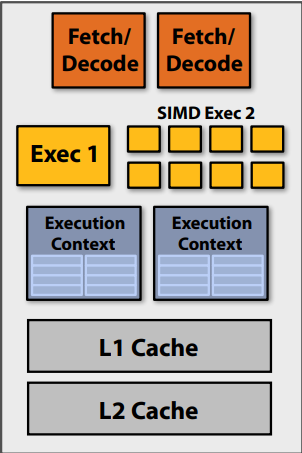
\includegraphics[width=0.25\textwidth]{figures/Single CPU Core.png}
    \caption{Single CPU Core}
    \label{fig:Single-Cpu-Core}
\end{figure}

\textbf{MASK}: How about the conditional executation? SIMD just operate 8 piceces simultaneously, we should specify or said, \textbf{SETTING MASK} to specify which elements we want to operate. The example showed in figure \ref{fig:MASK}.

\begin{figure}[h]
    \centering
    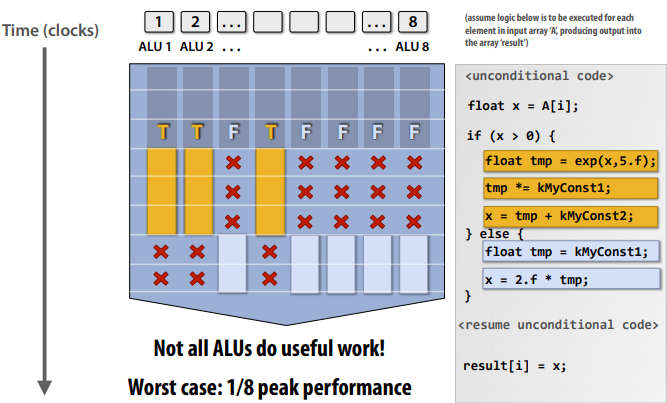
\includegraphics[width=0.75\textwidth]{figures/MASK.png}
    \caption{SIMD MASK}
    \label{fig:MASK}
\end{figure}

\subsection{Implementation}
Based on the set of instructions provided by CMU which located in \href{https://github.com/GiganticRay/CMU-418618HW/blob/main/asst1-f18/prog2_vecintrin/CMU418intrin.h}{CMU418intrin.h} and \href{https://github.com/GiganticRay/CMU-418618HW/blob/main/asst1-f18/prog2_vecintrin/CMU418intrin.cpp}{CMU418intrin.cpp}. My implementation of vector-adding in SIMD is located in \href{https://github.com/GiganticRay/CMU-418618HW/blob/main/asst1-f18/prog2_vecintrin/functions.cpp}{functions::clampedExpVector}.

\subsection{performance And Question Report}
Performance \& Question Report is located in \href{https://github.com/GiganticRay/CMU-418618HW/blob/main/asst1-f18/prog2_vecintrin/report2.txt}{GitHub report}.

\section{ISPC Experienment}
\subsection{Background}
\textbf{ISPC}--(Implicit Simple program multiple data Programing Compiler) is a compiler made by INTEL provide us an efficient way to implement SIMD prgrams running in the single/multiple cores. 

\subsection{Experienment Content}
The purpose is to get familar with ISPC by implement a program to caculate mandelbrot set. In ISPC program, \textbf{We assign data overall instead of assigning every data to each thread/execution unit explicitly} using keyword \textbf{forall}.

\subsection{Implementation}
The Ispc code is located in \href{https://github.com/GiganticRay/CMU-418618HW/blob/main/asst1-f18/prog3_mandelbrot_ispc/mandelbrot.ispc}{mandelbrot.iscp}.

\subsection{Result Report}
Result Report is located in \href{https://github.com/GiganticRay/CMU-418618HW/blob/main/asst1-f18/prog3_mandelbrot_ispc/report.txt}{report.txt}

\subsubsection{Determine how many tasks to creat And Cope with Bound area}
A: using script to change the parameter of threadCount, Drawing graph based on these different threadCount to get the optimize point.
    Dealing with the situation that the rows in the image is not divisible by the number of tasks.
    
A: EASY!!! check out mandelbrot.ispc::mandelbrot\_ispc\_task, it has already copying with the fontier of last segment, so what we need to do in mandelbrot.ispc::mandelbrot\_ispc\_withtasks is only determine whether adding or not a thread which used to caculate the extra part of data.

\subsubsection{the difference bwtween foreach and launch}
In terms of my view from now on, foreach is running just like the serial function. the difference bwtween serial and foreach is their running CPU, the first is common cpu, the latter is vector cpu. The reason that vector cpu could sppedup is that the cooprating unit in vector cpu is VECTOR. LAUNCH is more like creating multiple threads running on different cores. so it's at the same level of multiple threads. From simplicity, foreach is still a single thread, LAUNCH is already in the level of multiple threads.


% If you don't cite any references, please comment the following two lines
% \bibliographystyle{ieee}
% \bibliography{ref.bib}

\end{document}